\begin{figure}
  \centering

  \begin{minipage}{0.9\textwidth}
    \raggedleft
    \begin{tikzpicture}
      \node (table) [matrix,row sep=1.5*\nodeheight,column sep=-\pgflinewidth] {
        \node (plaintext1) [smallrect] {$m_1$}; & \node (plaintext2) [smallrect] {$m_2$}; & \node (plaintext3) [smallrect] {$m_3$}; & \node (plaintext4) [smallrect] {$m_4$}; \\
        \node (encryption1) [circle] {$E_K$}; & \node (encryption2) [circle] {$E_K$}; & \node (encryption3) [circle] {$E_K$}; & \node (encryption4) [circle] {$E_K$}; \\
        \node (ciphertext1) [smallrect] {$c_1$}; & \node (ciphertext2) [smallrect] {$c_2$}; & \node (ciphertext3) [smallrect] {$c_3$}; & \node (ciphertext4) [smallrect] {$c_4$}; \\
      };
      \path [line] (plaintext1) -- (encryption1);
      \path [line] (plaintext2) -- (encryption2);
      \path [line] (plaintext3) -- (encryption3);
      \path [line] (plaintext4) -- (encryption4);
      \path [line] (encryption1) -- (ciphertext1);
      \path [line] (encryption2) -- (ciphertext2);
      \path [line] (encryption3) -- (ciphertext3);
      \path [line] (encryption4) -- (ciphertext4);

      \node (table2) [matrix,right=1 of table,row sep=\nodeheight,column sep=\nodeheight] {
        \node (plaintext) {
\includegraphics[scale=0.25]{images/tux.jpg}}; \\
        \node (ciphertext) {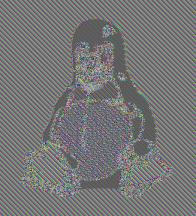
\includegraphics[scale=0.25]{images/tux-ecb.jpg}}; \\
      };
      \path [line] (plaintext) -- (ciphertext);
    \end{tikzpicture}
    \subcaption{ECB block mode}
  \end{minipage}
  \begin{minipage}{0.9\textwidth}
    \raggedleft
    \begin{tikzpicture}
      \node (table) [matrix,row sep=1.5*\nodeheight,column sep=-\pgflinewidth] {
        & \node (plaintext1) [smallrect] {$m_1$}; & \node (plaintext2) [smallrect] {$m_2$}; & \node (plaintext3) [smallrect] {$m_3$}; & \node (plaintext4) [smallrect] {$m_4$}; \\[-0.75*\nodeheight]
        \node (iv) [smallrect] {$IV$}; & \node (plaintext1_after) [inner sep=0] {\Large $\oplus$}; & \node (plaintext2_after) [inner sep=0] {\Large $\oplus$}; & \node (plaintext3_after) [inner sep=0] {\Large $\oplus$}; & \node (plaintext4_after) [inner sep=0] {\Large $\oplus$}; \\[-0.75*\nodeheight]
        & \node (encryption1) [circle] {$E_K$}; & \node (encryption2) [circle] {$E_K$}; & \node (encryption3) [circle] {$E_K$}; & \node (encryption4) [circle] {$E_K$}; \\[-0.75*\nodeheight]
        & \coordinate (ciphertext1_before) [inner sep=0]; & \coordinate (ciphertext2_before) [inner sep=0]; & \coordinate (ciphertext3_before) [inner sep=0]; & \coordinate (ciphertext4_before) [inner sep=0]; \\[-0.75*\nodeheight]
        & \node (ciphertext1) [smallrect] {$c_1$}; & \node (ciphertext2) [smallrect] {$c_2$}; & \node (ciphertext3) [smallrect] {$c_3$}; & \node (ciphertext4) [smallrect] {$c_4$}; \\
      };
      \path [line] (plaintext1) -- (plaintext1_after);
      \path [line] (plaintext2) -- (plaintext2_after);
      \path [line] (plaintext3) -- (plaintext3_after);
      \path [line] (plaintext4) -- (plaintext4_after);
      \path [line] (plaintext1_after) -- (encryption1);
      \path [line] (plaintext2_after) -- (encryption2);
      \path [line] (plaintext3_after) -- (encryption3);
      \path [line] (plaintext4_after) -- (encryption4);
      \path [line] (encryption1) -- (ciphertext1);
      \path [line] (encryption2) -- (ciphertext2);
      \path [line] (encryption3) -- (ciphertext3);
      \path [line] (encryption4) -- (ciphertext4);
      \path [line] (iv) -- (plaintext1_after);
      \path [line] (ciphertext1_before) -| ($(encryption1) !.5! (encryption2)$) |- (plaintext2_after);
      \path [line] (ciphertext2_before) -| ($(encryption2) !.5! (encryption3)$) |- (plaintext3_after);
      \path [line] (ciphertext3_before) -| ($(encryption3) !.5! (encryption4)$) |- (plaintext4_after);

      \node (table2) [matrix,right=1 of table,row sep=\nodeheight,column sep=\nodeheight] {
        \node (plaintext) {
\includegraphics[scale=0.25]{images/tux.jpg}}; \\
        \node (ciphertext) {
\includegraphics[scale=0.25]{images/tux-cbc.jpg}}; \\
      };
      \path [line] (plaintext) -- (ciphertext);
    \end{tikzpicture}
    \subcaption{CBC block mode}
    \bigskip
  \end{minipage}

  \begin{footnotesize}
    The ECB mode is the most basic block mode, which does not perform any block feedback. Note that the plaintext structure is still observable in the ciphertext.
  \end{footnotesize}

  \caption{Basic block modes}
  \label{figure/block-modes}
\end{figure}
